%<*figvecfields>
\begin{figure}
    \centering
    \newcommand*{\subfigwidth}{.49\textwidth}
    \begin{subfigure}[b]{\subfigwidth}
        \centering
        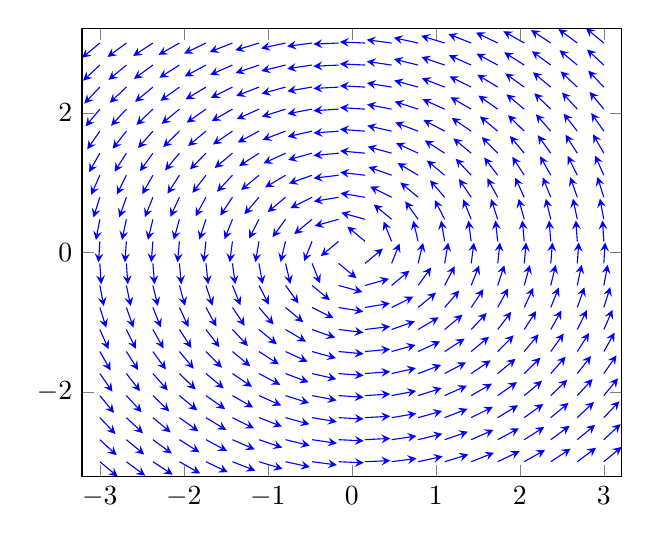
\begin{tikzpicture}
            \def\length{.5*sqrt(x^2+y^2)}
            \begin{axis}[domain=-3:3, view={0}{90}]
                \addplot3[blue, quiver={u={-y/(\length)}, v={x/(\length)}, scale arrows=0.15}, -stealth,samples=20] {0};
            \end{axis}
        \end{tikzpicture}
        \caption{
            \(
            \begin{bmatrix}
                \frac{-y}{\sqrt{x^2+y^2}} & \frac{x}{\sqrt{x^2+y^2}}
            \end{bmatrix}
            \)
        }\label{subfig:vecfield1}
    \end{subfigure}
    \vskip\baselineskip
    \begin{subfigure}[b]{\subfigwidth}
        \centering
        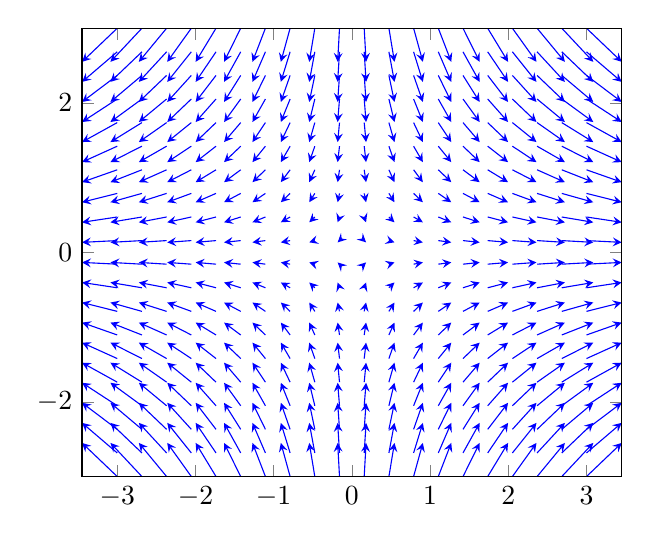
\begin{tikzpicture}
            \begin{axis}[domain=-3:3, view={0}{90}]
                \addplot3[blue, quiver={u={x}, v={-y}, scale arrows=0.15}, -stealth,samples=20] {0};
            \end{axis}
        \end{tikzpicture}
        \caption{
            \(
            \begin{bmatrix}
                x & y
            \end{bmatrix}
            \)
        }\label{subfig:vecfield2}
    \end{subfigure}
    \caption{Vector fields.}\label{fig:vectorfields}
\end{figure}
%</figvecfields>

%<*contouterintegral>
%</contourintegral>